\documentclass[12pt]{article}
\usepackage[margin=2cm]{geometry} 
\usepackage{titling}
\usepackage{graphicx}
\usepackage{float}
\usepackage[hidelinks]{hyperref}
\usepackage[italian]{babel}

\setlength\parindent{0pt}
\setlength{\parskip}{1em}
\setlength{\droptitle}{-2cm}

\title{Istruzioni d'uso Thymio}
\author{Università della Svizzera Italiana}
\date{Versione \today \ (Thymio Suite 2.0.0)}


\begin{document}
\maketitle
\tableofcontents
\newpage


\section{Installazione}\label{installation}

	\subsection{Windows}
	
		Recarsi all'indirizzo \url{https://www.thymio.org/it/programma} e scaricare il software Thymio Suite cliccando sul bottone \texttt{Download} sotto il logo Windows. Prestare attenzione a scegliere la versione adatta al proprio sistema (32/64 bit).\\
		Aprire il file .exe scaricato e proseguire con l'installazione guidata. Al primo avvio dell'applicazione potrebbe essere necessario autorizzarla ad accedere a internet: cliccare su "Consenti accesso" nella finestra di dialogo di Windows Firewall.
		
	\subsection{MacOS}
	
		Recarsi all'indirizzo \url{https://www.thymio.org/it/programma} e scaricare il software Thymio Suite cliccando sul bottone \texttt{Download} sotto il logo Apple.\\	
		Aprire il file .dmg scaricato e trascinare il file ThymioSuite.app in Applicazioni.
		
	\subsection{Linux}
	
		Recarsi all'indirizzo \url{https://www.thymio.org/it/aiuto/linux-installation/} e seguire le istruzioni per la piattaforma in uso.
			

\section{Collegamento del robot}

	Prima di utilizzare qualsiasi software, è necessario collegare almeno un robot al computer (vedi sezione \ref{multi-robot} per multipli robot). Questo può essere fatto in due modi: tramite cavo o wireless (se supportato).
	
	\subsection{Cavo USB}
	
		Collegare il cavo in dotazione ad una porta libera sulla propria macchina e alla porta microUSB sul retro del Thymio. Il robot si accenderà automaticamente non appena rilevata la connessione.
		
	\subsection{Dongle wireless (se disponibile)}
	
		Collegare il dongle ad una porta libera sulla propria macchina e accendere il robot tenendo premuto il tasto centrale per circa 3 secondi. Il LED del dongle e del robot dovrebbero lampeggiare alla stessa frequenza.
	

\section{Software}

	Tutti i programmi necessari per configurare e programmare Thymio sono raccolti in una sola applicazione, Thymio Suite.
	
	\begin{figure}[H]
		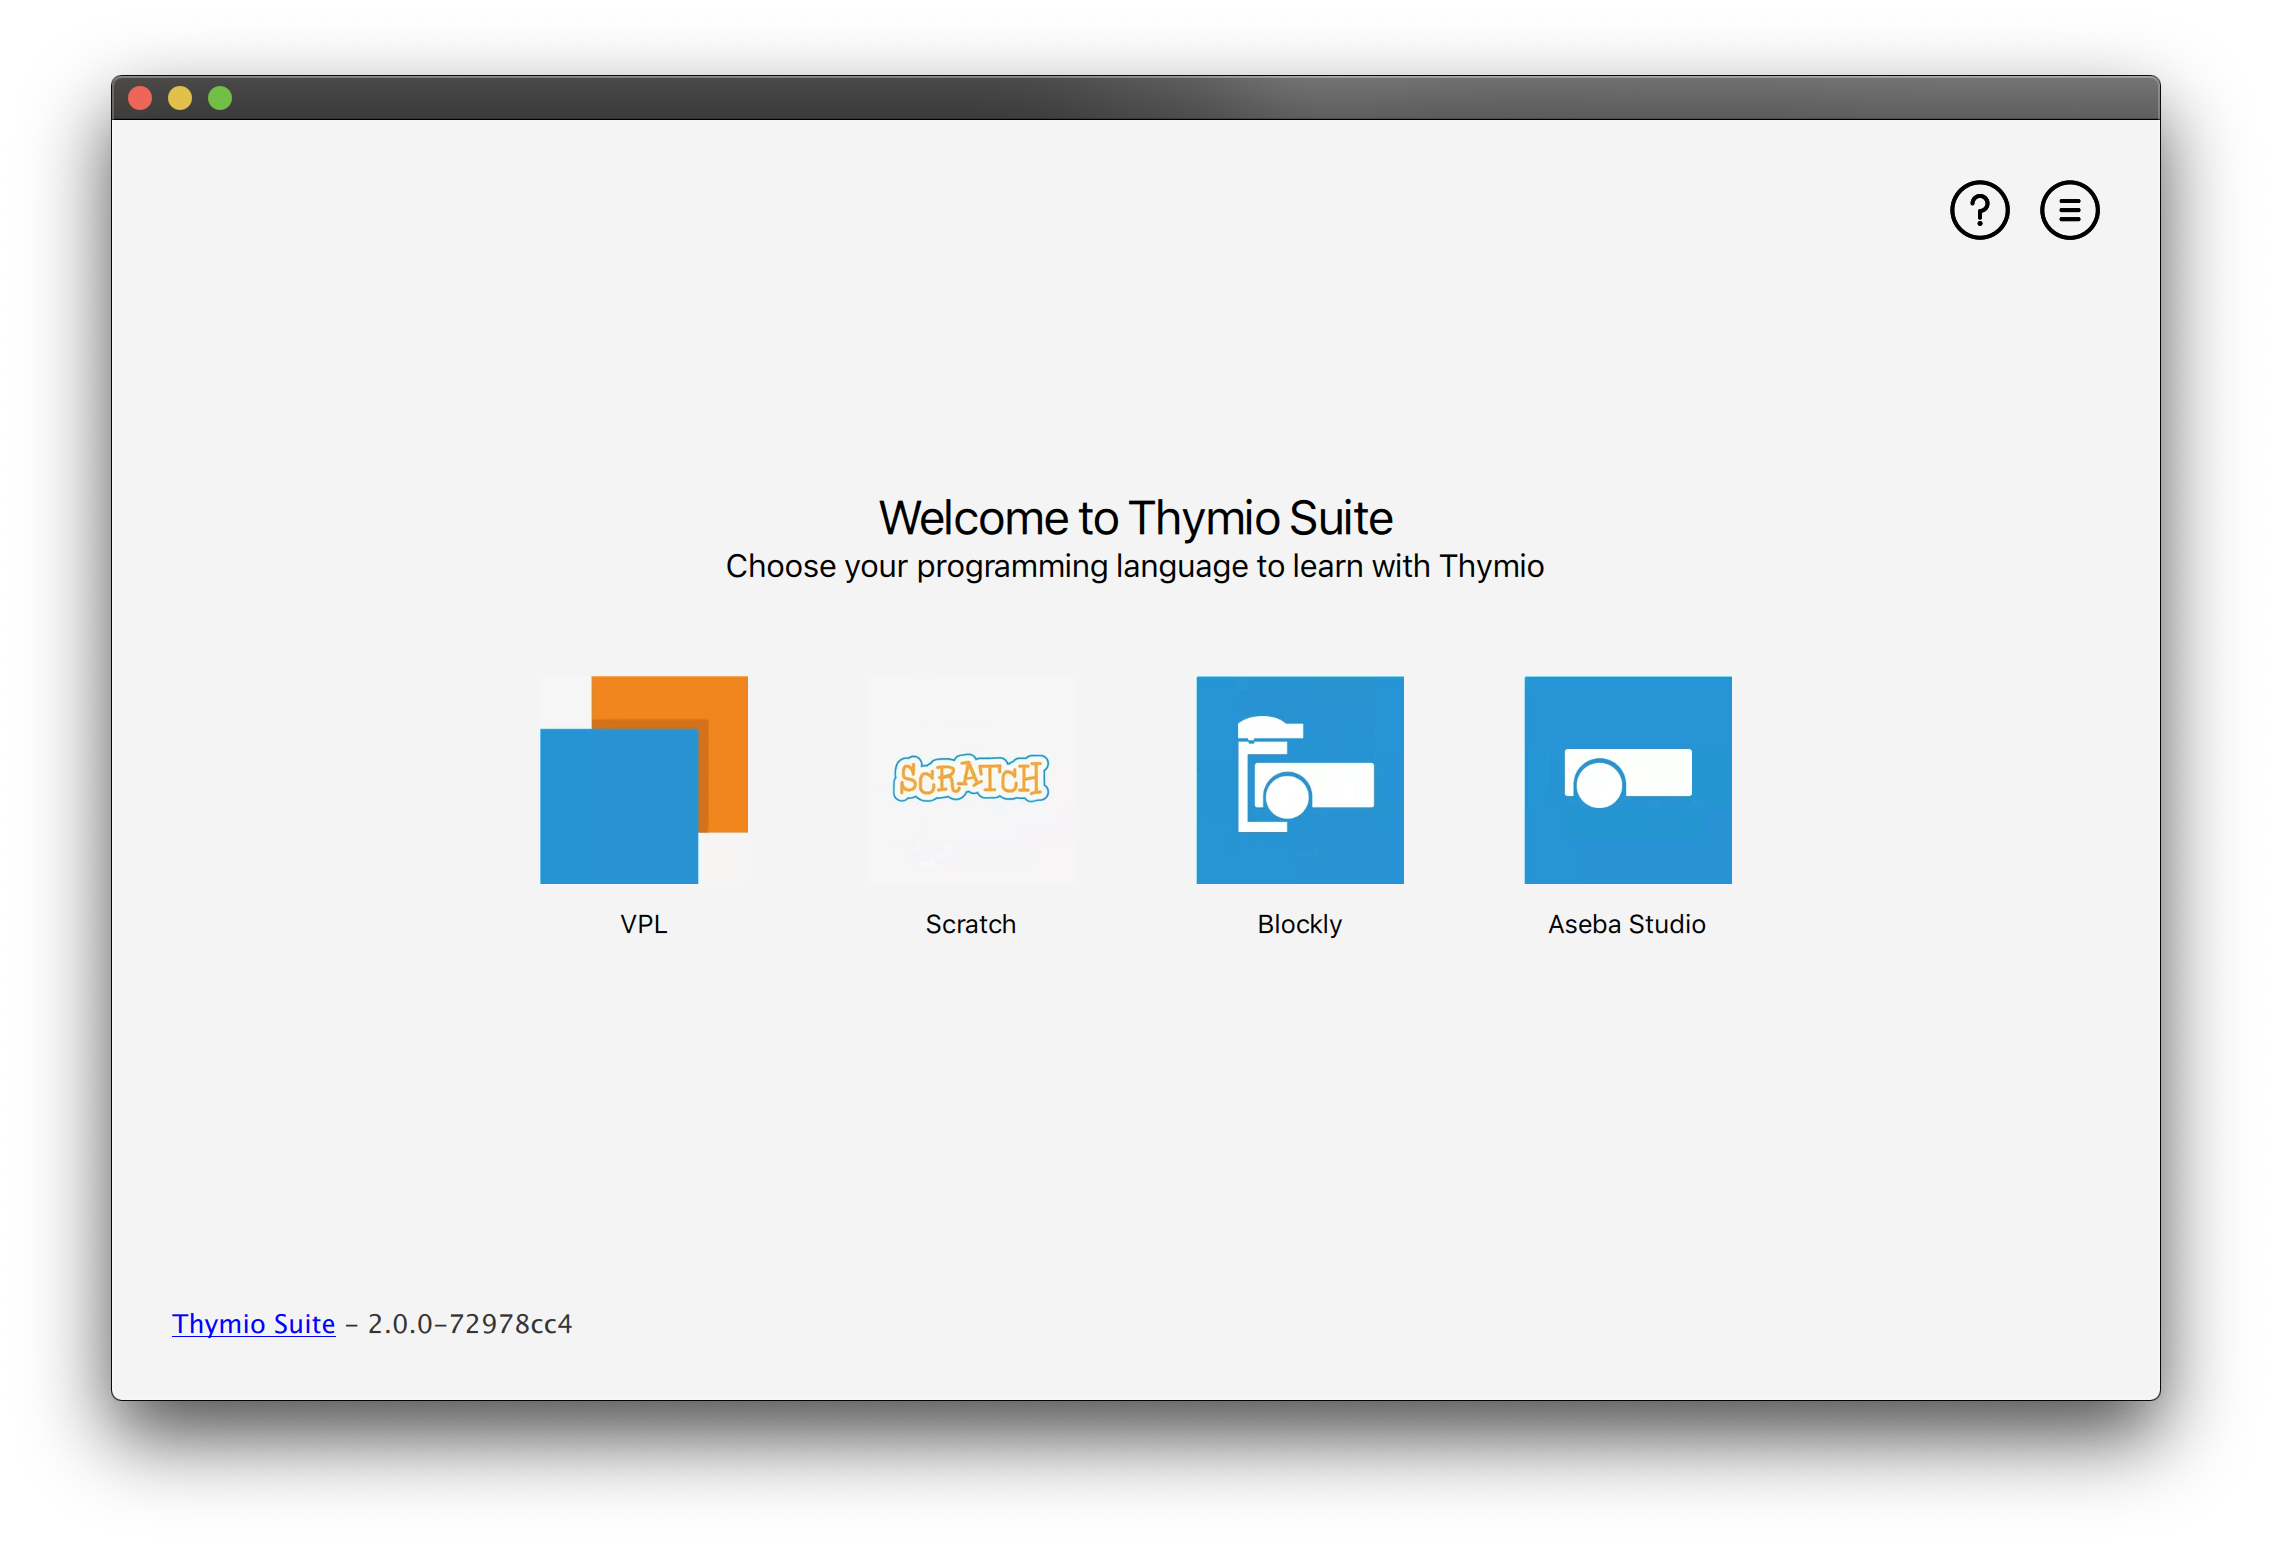
\includegraphics[width=\textwidth]{img/thymioSuite.png}
		\caption{La finestra principale di Thymio Suite}
		\label{aseba1}
	\end{figure}
	
	Nota: in caso Blockly, VPL e Scratch non dovessero aprirsi al click della relativa icona, recarsi nel menu a destra e deselezionare la casella \texttt{Usa il browser di sistema}.
	
	Nota: su MacOS il programma verrà bloccato dal sistema siccome proviene da una fonte esterna (vedi figura \ref{macErr}). Cliccare su Annulla, in seguito recarsi in Impostazioni di Sistema, sotto Sicurezza e Privacy e cliccare su Apri Comunque. Ora è possibile avviare il software, cliccando un'ultima volta su Apri quando richiesto. Altri avvisi appariranno lanciando Blockly e le altre applicazioni, ma sarà sufficiente cliccare su Apri.
		
	\begin{figure}[H]
		\centering
			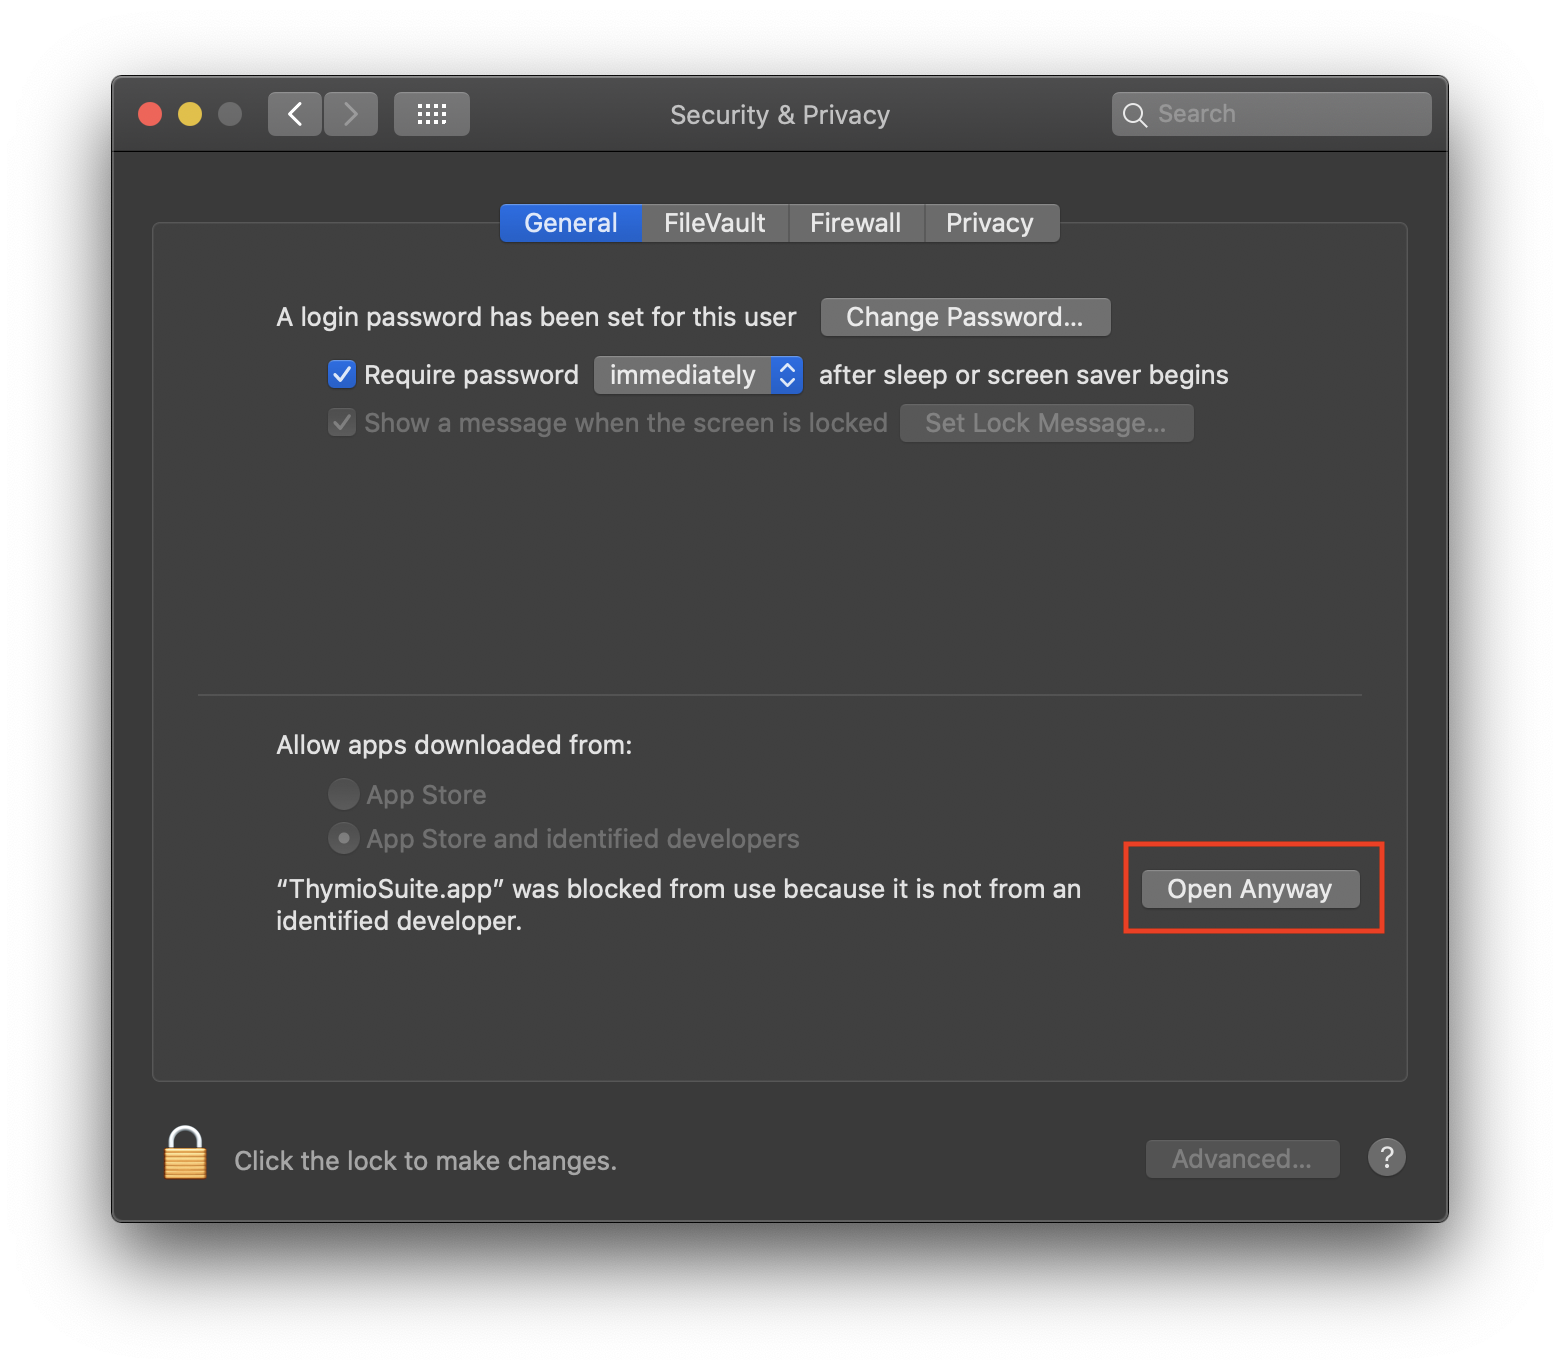
\includegraphics[width=0.7\textwidth]{img/macWarn.png}
			\caption{Le Impostazioni di Sistema di MacOS}
			\label{macErr}
	\end{figure}
		
	\subsection{Aseba Studio}
	
		Aseba Studio è un software per programmare direttamente i robot Thymio, pensato per utenti più esperti. Per utilizzarlo è sufficiente lanciare Thymio Suite e cliccare su Aseba Studio. Scegliere un robot dalla lista e premere su \texttt{Programma con Aseba Studio}.
		
		\begin{figure}[H]
			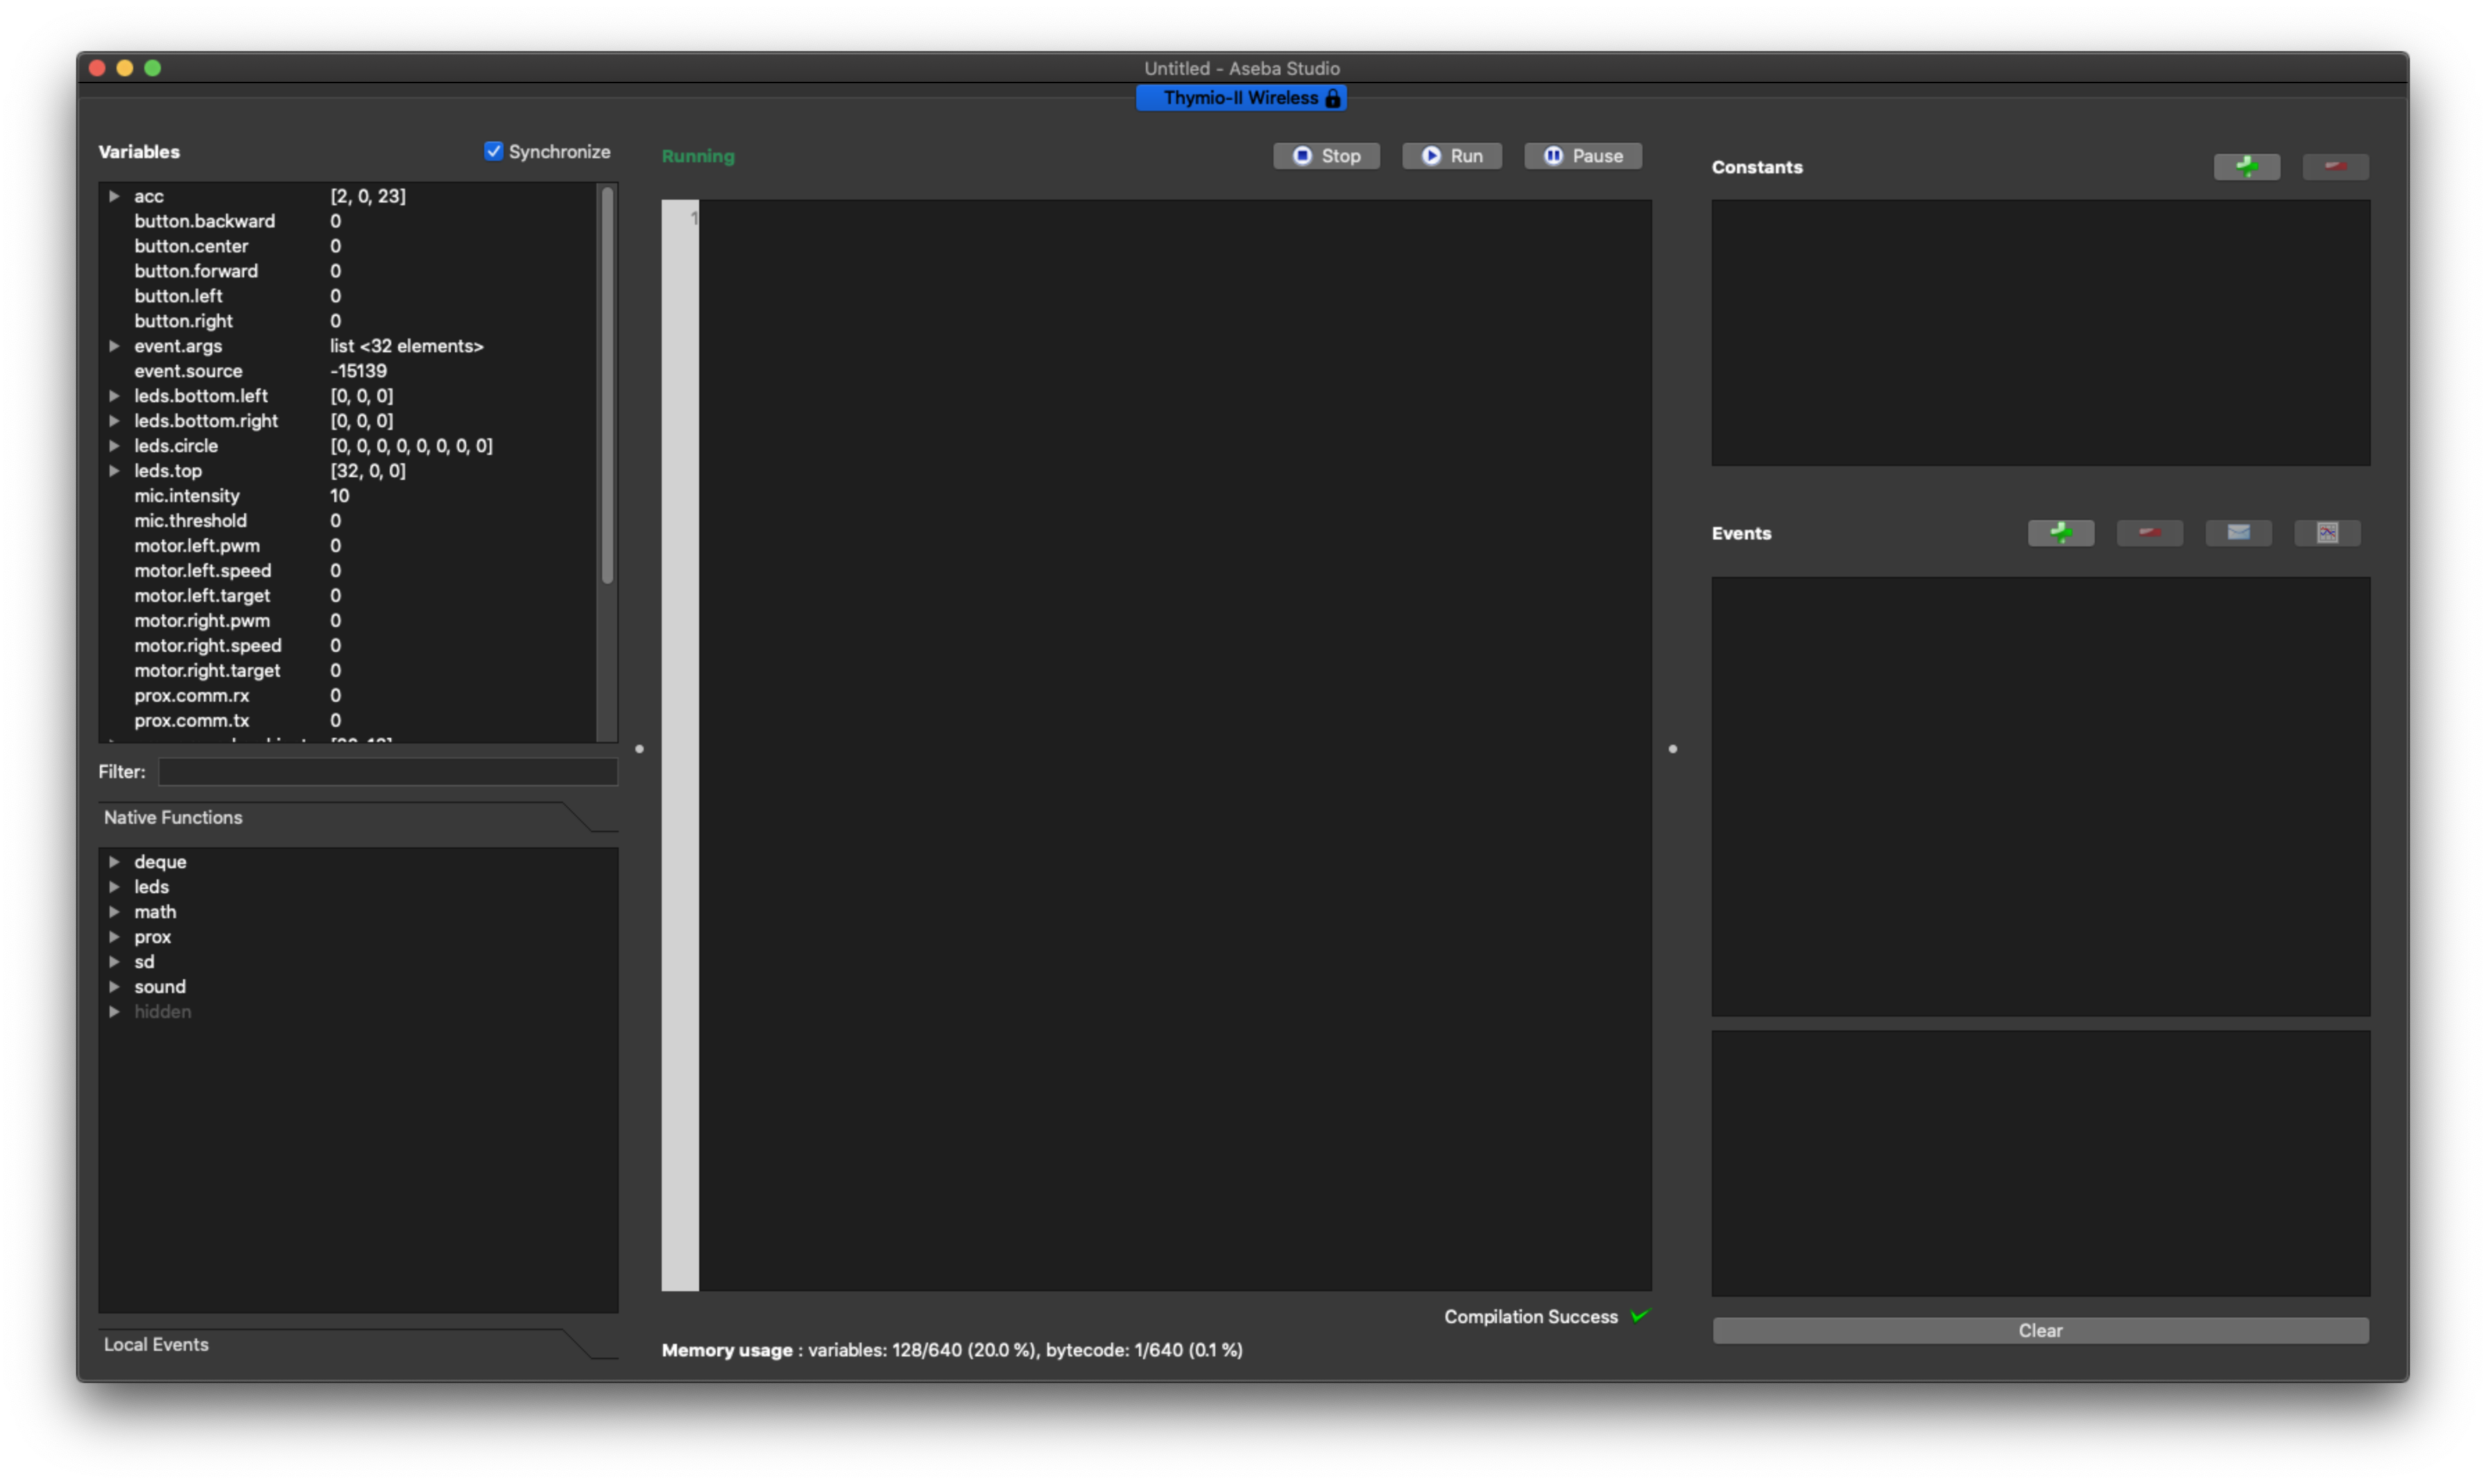
\includegraphics[width=\textwidth]{img/asebaStudio.png}
			\caption{La finestra principale di Aseba Studio}
			\label{main_aseba}
		\end{figure}		

	\subsection{Blockly}

		Blockly è un software per programmare in maniera intuitiva. Per utilizzarlo è sufficiente lanciare Thymio Suite e cliccare su Blockly. Scegliere un robot dalla lista e premere su \texttt{Programma con Blockly}.
		
		\begin{figure}[H]
			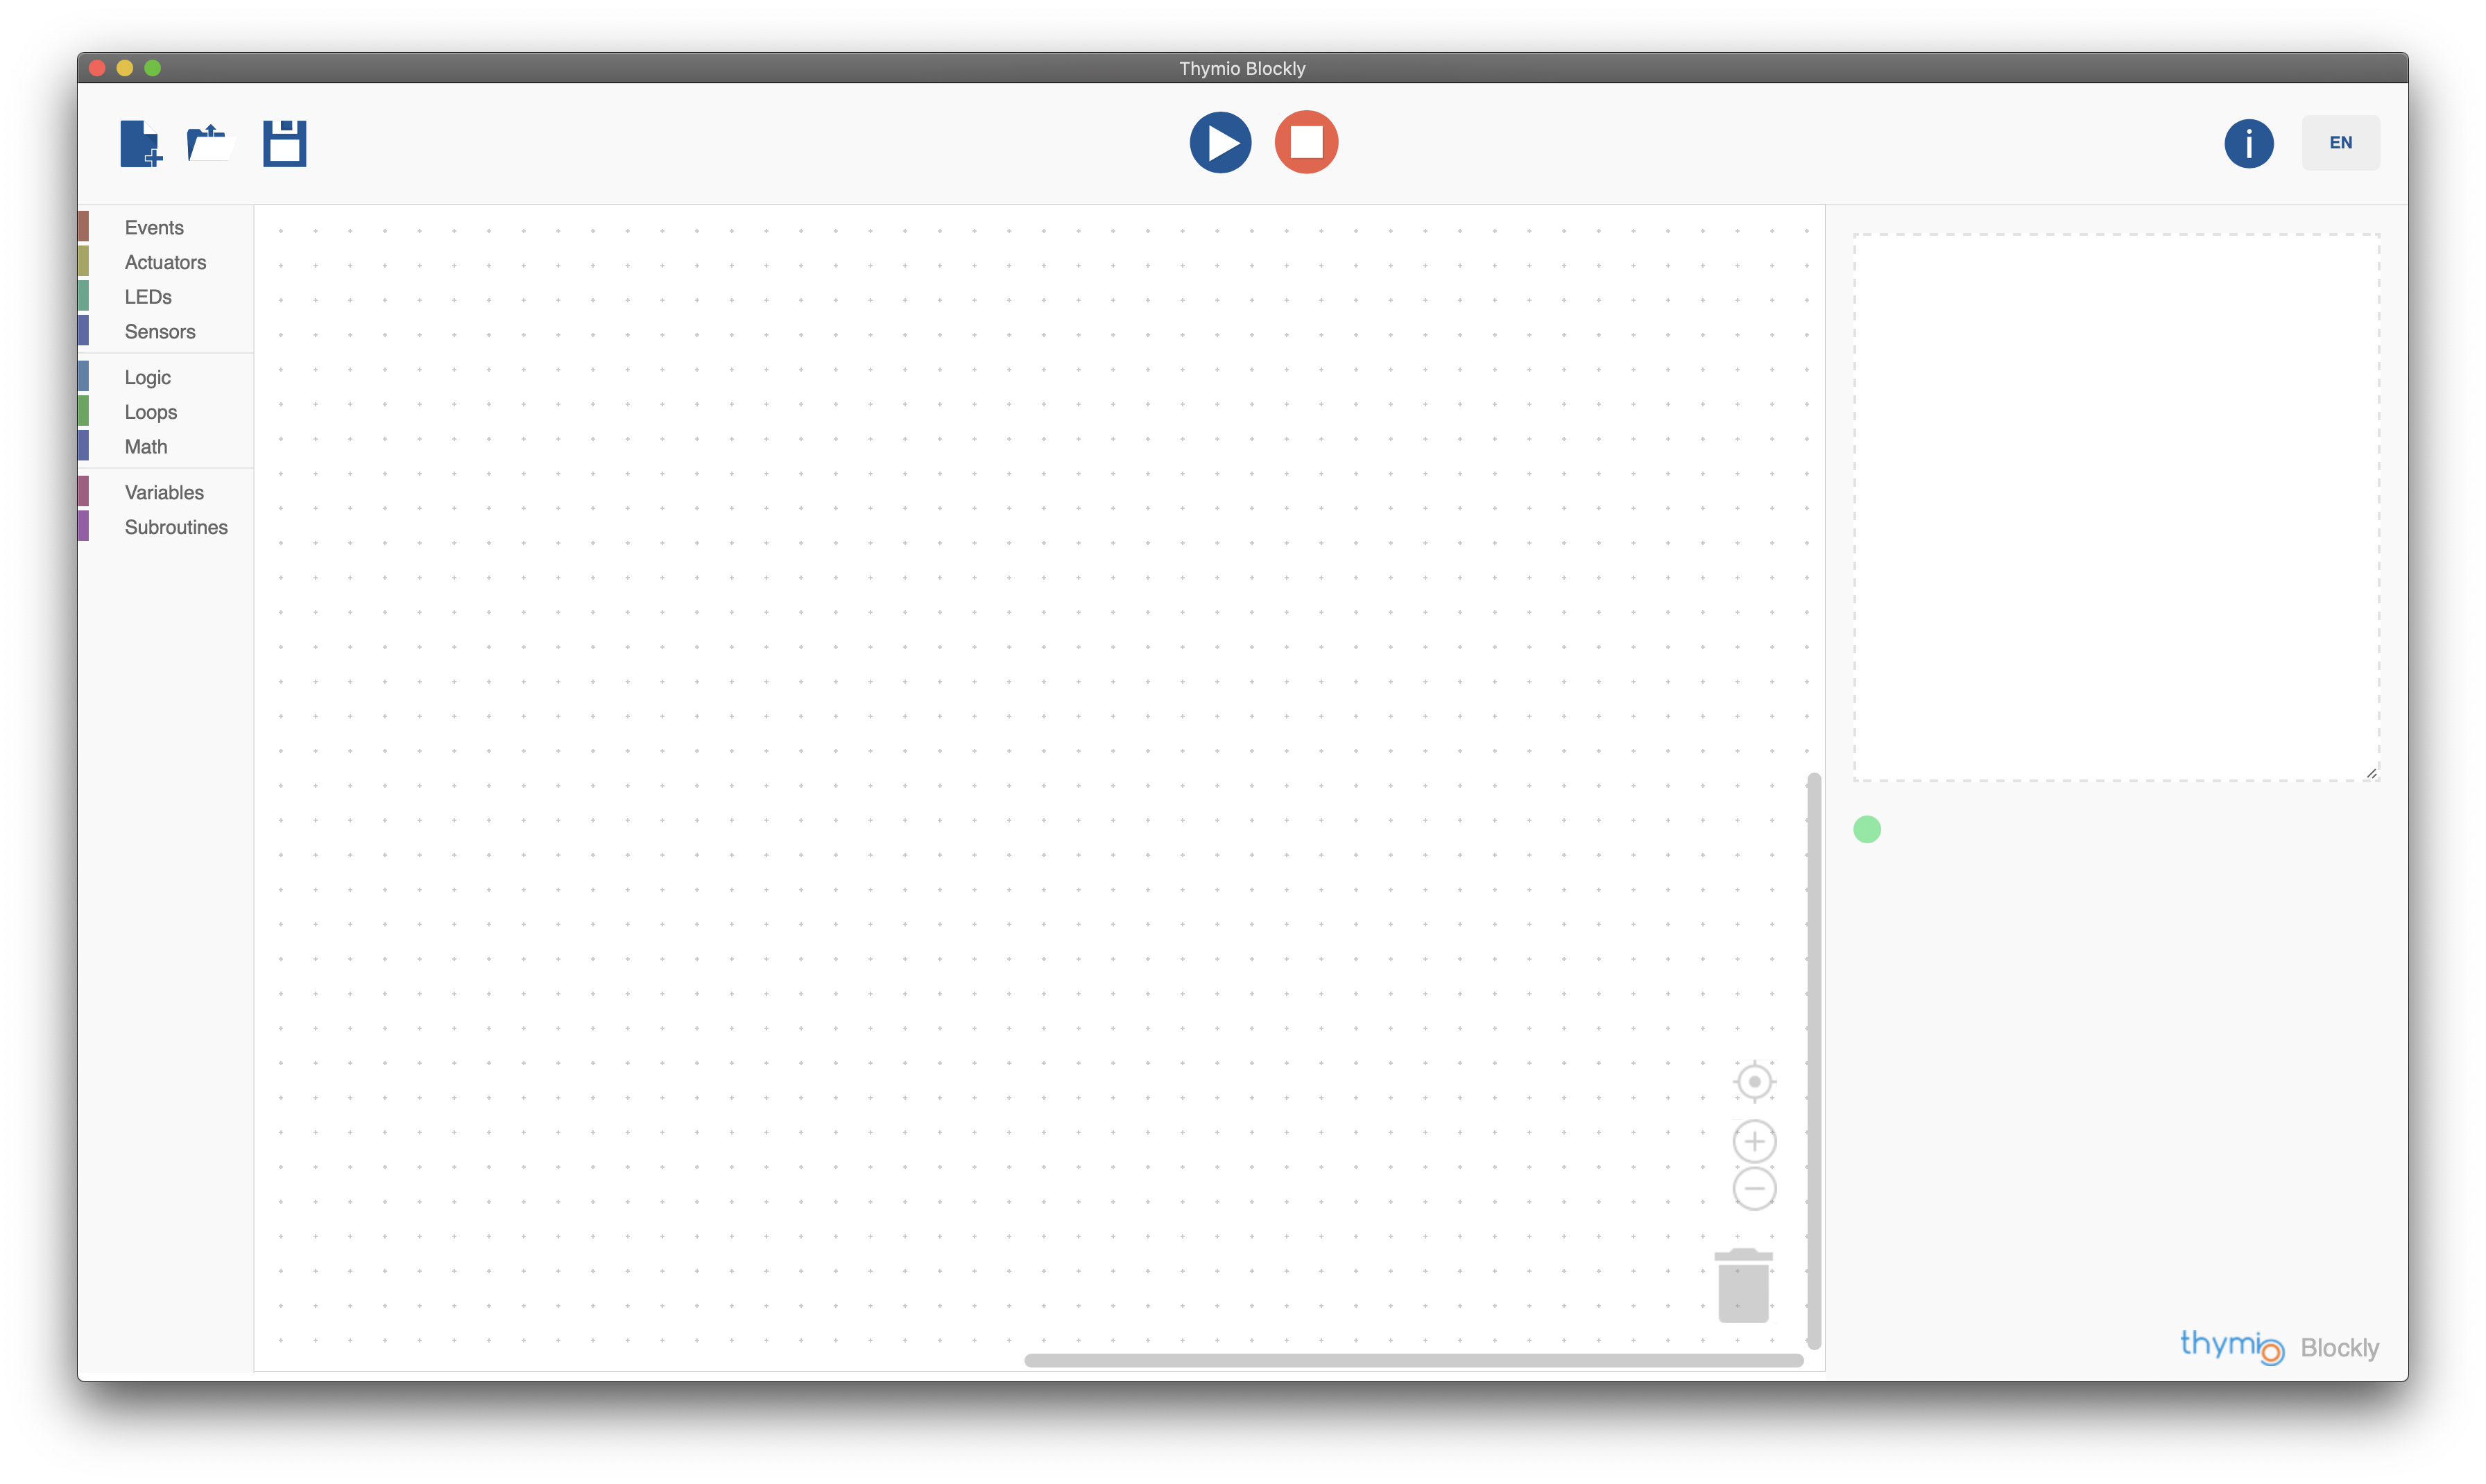
\includegraphics[width=\textwidth]{img/blockly.png}
			\caption{La finestra principale di Blockly}
			\label{main_blockly}
		\end{figure}
		
	\subsection{VPL}
	
		VPL (Visual Programming Language) è un software semplificato pensato per i più giovani. Per utilizzarlo è sufficiente lanciare Thymio Suite e cliccare su VPL. Scegliere un robot dalla lista e premere su \texttt{Programma con VPL}.
		
		\begin{figure}[H]
			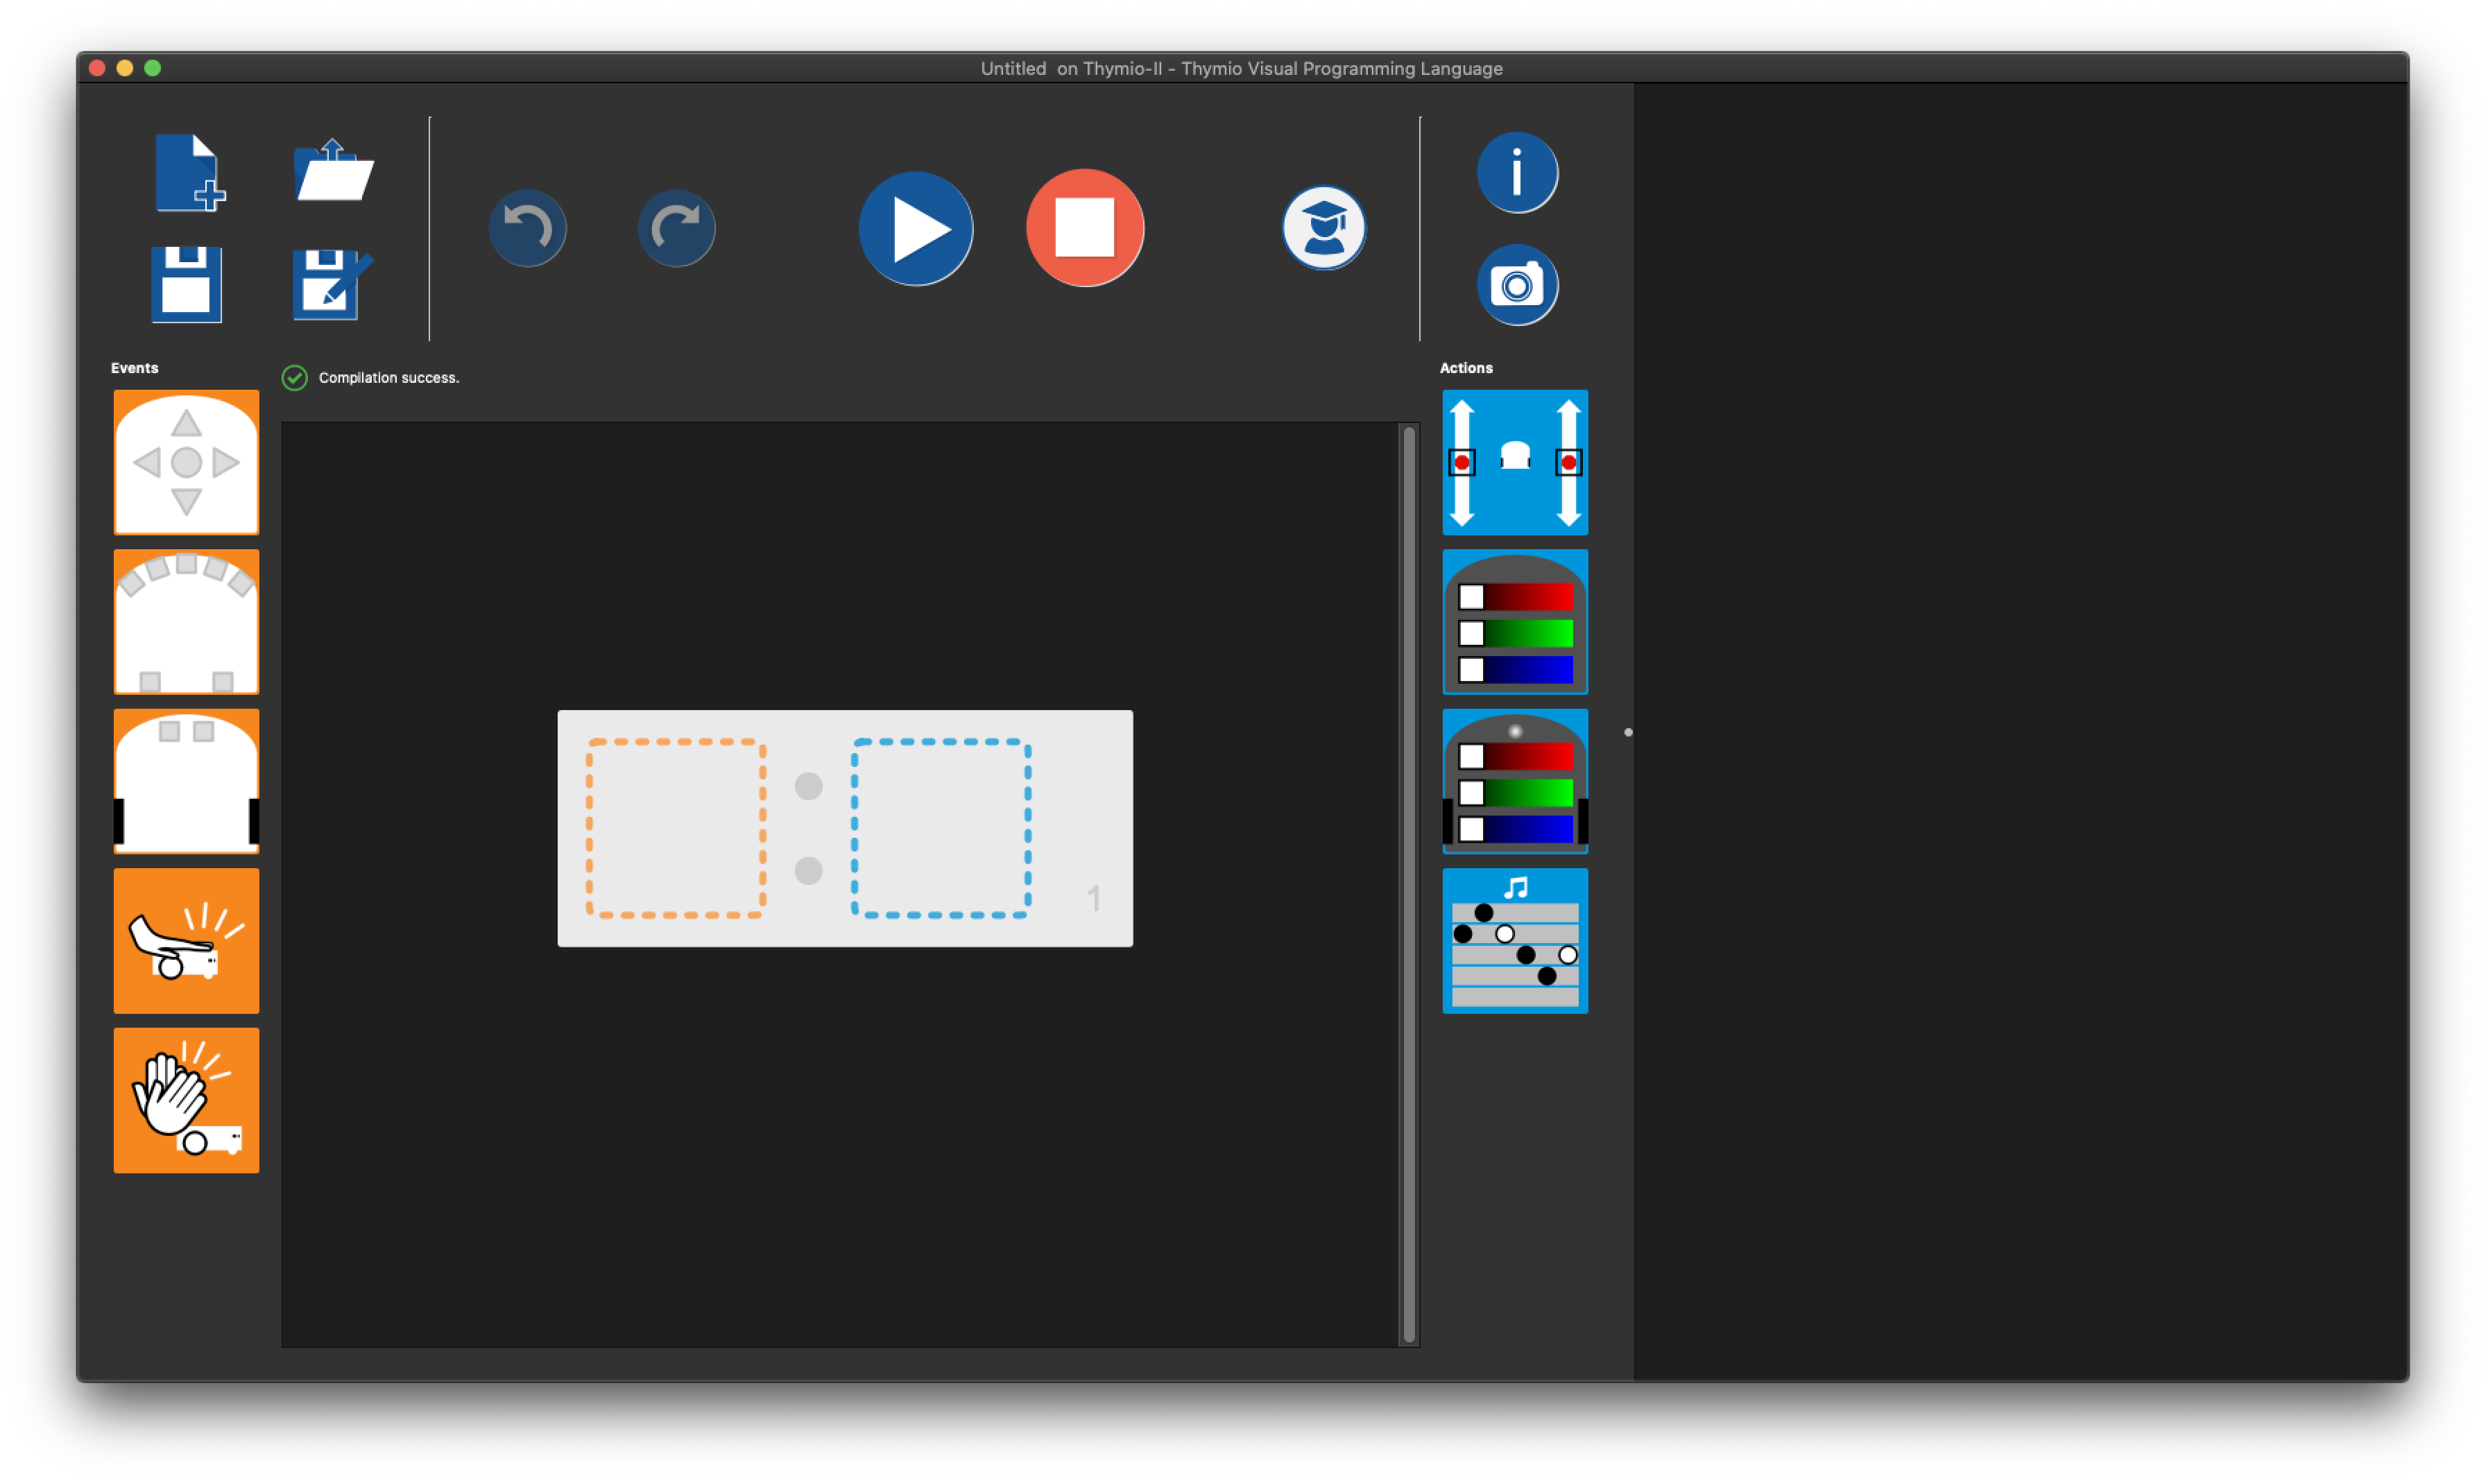
\includegraphics[width=\textwidth]{img/vpl.png}
			\caption{La finestra principale di VPL}
			\label{main_vpl}
		\end{figure}
		
	\subsection{Scratch}
	
		Scratch è un linguaggio educativo sviluppato dal MIT (sito ufficiale: \url{https://scratch.mit.edu/}). Per utilizzarlo è sufficiente lanciare Thymio Suite e cliccare su Scratch. Scegliere un robot dalla lista e premere su \texttt{Programma con Scratch}.
		
		\begin{figure}[H]
			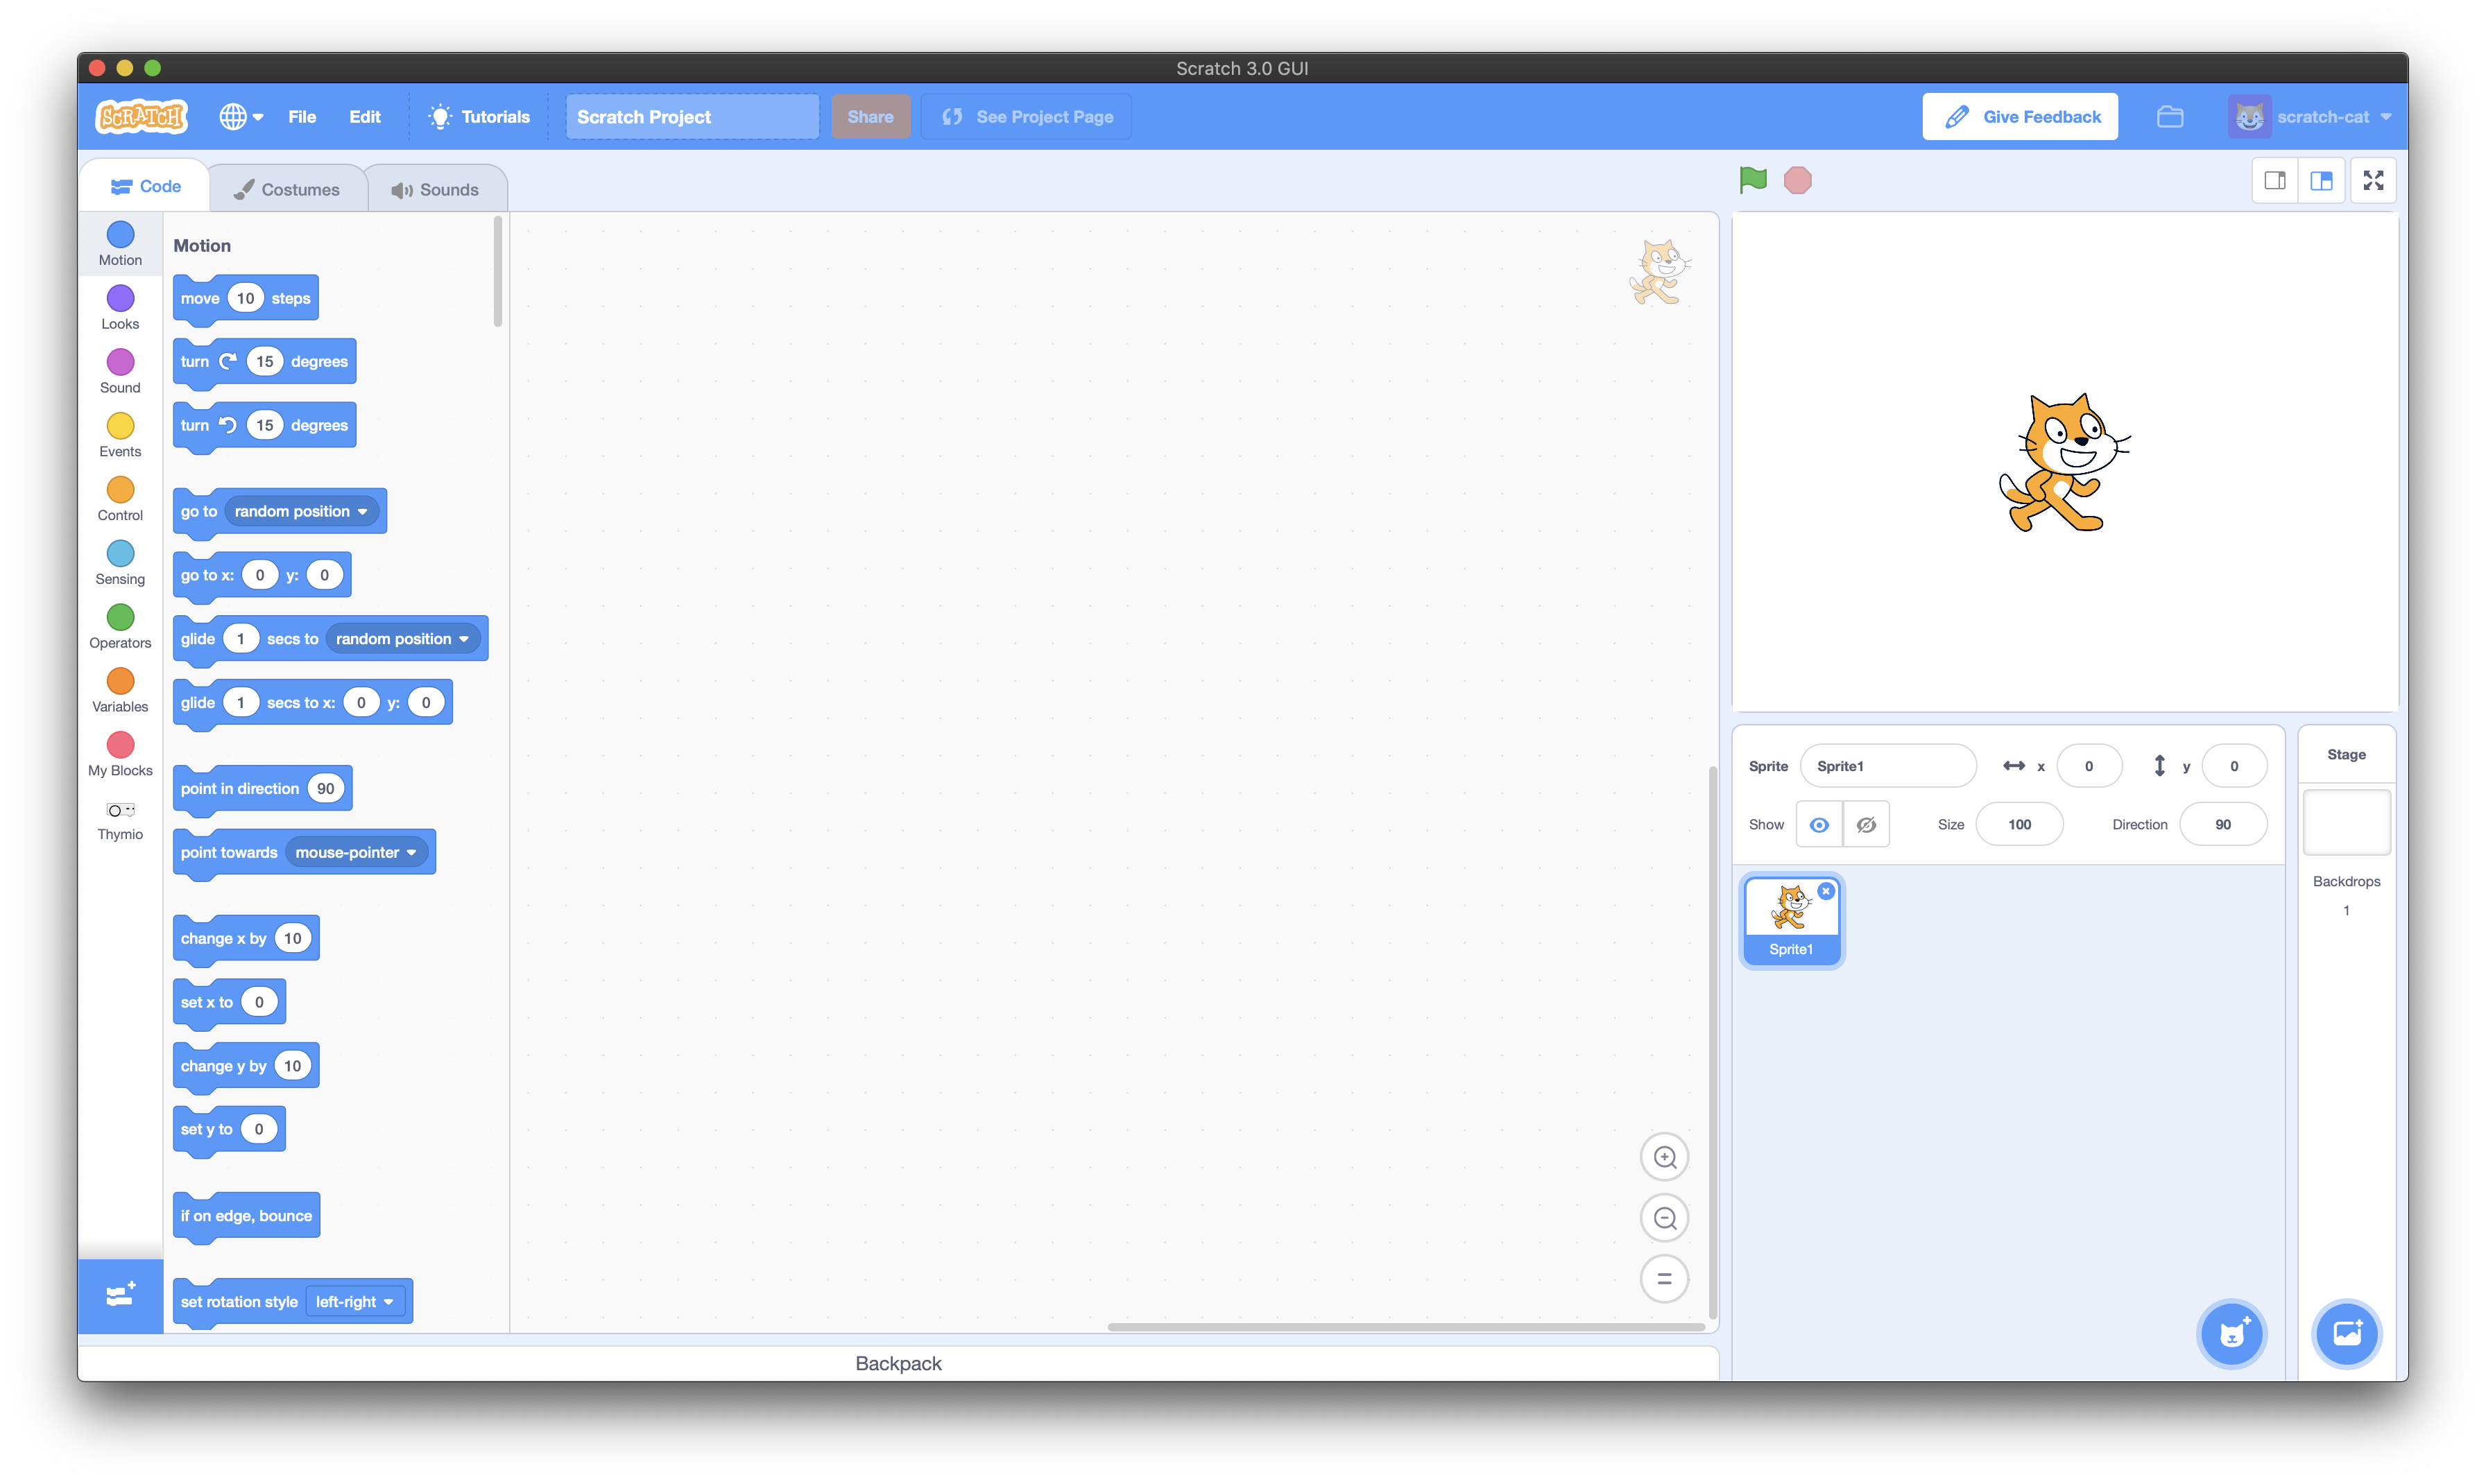
\includegraphics[width=\textwidth]{img/scratch.png}
			\caption{La finestra principale di Scratch}
			\label{main_scratch}
		\end{figure}
		
	\subsection{Thymio Simulator}
	
		No Thymio? No problem! Esiste un simulatore previsto per emulare uno o più robot sul proprio computer, incluso con il software scaricato al punto \ref{installation}.
		
		Per utilizzarlo è necessario scaricare le mappe disponibili all'indirizzo \url{https://www.thymio.org/thymio-simulator}. Dopodiché è sufficiente selezionare \texttt{Lancia un simulatore} dal menu a destra e scegliere la mappa desiderata; in seguito, selezionare il software di programmazione desiderato dall'applicazione principale.
		I robot presenti nella simulazione saranno elencati come se fossero collegati al proprio computer e sarà possibile iniziare a programmarli.
		
		
\section{Esempi di codice}

	\subsection{USI Showroom}
		
		Al seguente indirizzo sono disponibili diversi file con esempi di semplici programmi appositamente prodotti dall'USI:
		
		\url{https://github.com/USI-Showroom/thymio/examples}
		
		
		- easyBlackLine: un semplice programma per far seguire a Thymio una linea nera con i due sensori inferiori
		
		- ledTest: accende tutti i LED presenti sul robot
		
		- remoteDrive: un progetto per controllare il movimento di un Thymio tramite un altro (richiede due robot)
		
	
	\subsection{Risorse ufficiali}
	
		Ai seguenti indirizzi sono disponibili diversi tutorial ed esempi ufficiali di codice:
	
		\url{http://wiki.thymio.org/en:creations}
		
		\url{https://github.com/Mobsya/thymio-programming-exercises}
		
		\url{https://github.com/Mobsya/thymio-vpl-tutorial}
	
	
\section{Comunicazione fra robot}\label{network}

	È possibile far comunicare due robot tramite infrarossi (IR). Siccome la comunicazione avviene tramite i sensori orizzontali (cinque anteriori e due posteriori), i robot devono essere in grado di ``vedersi''.
	
	Prima di tutto è necessario attivare la comunicazione IR su entrambi i robot, dopodiché si possono usare i blocchi o i comandi specialmente previsti (rispettivamente su Blockly e Aseba studio) per trasmettere e ricevere i segnali; purtroppo al momento questa funzione non è disponibile in VPL. 
	
	Di seguito un semplice esempio dove il primo robot trasmette un segnale IR e il secondo reagisce cambiando il colore del LED superiore: 
	
	\begin{figure}[H]
		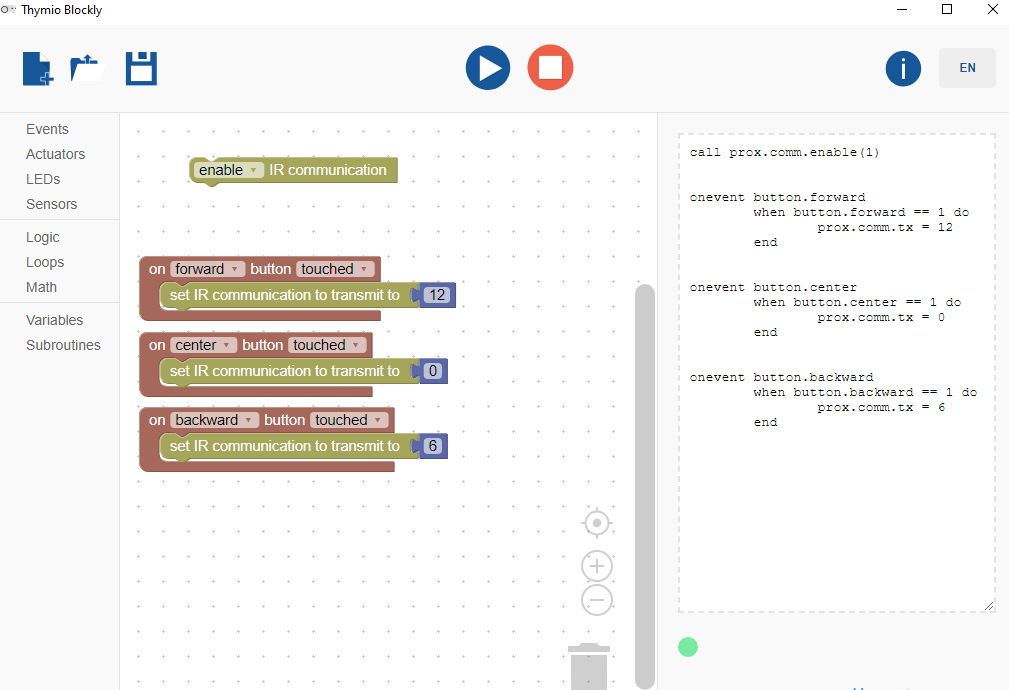
\includegraphics[width=\textwidth]{img/blocklyIR1.png}
		\label{blocklyIR1}
	\end{figure}
		
	\begin{figure}[H]
		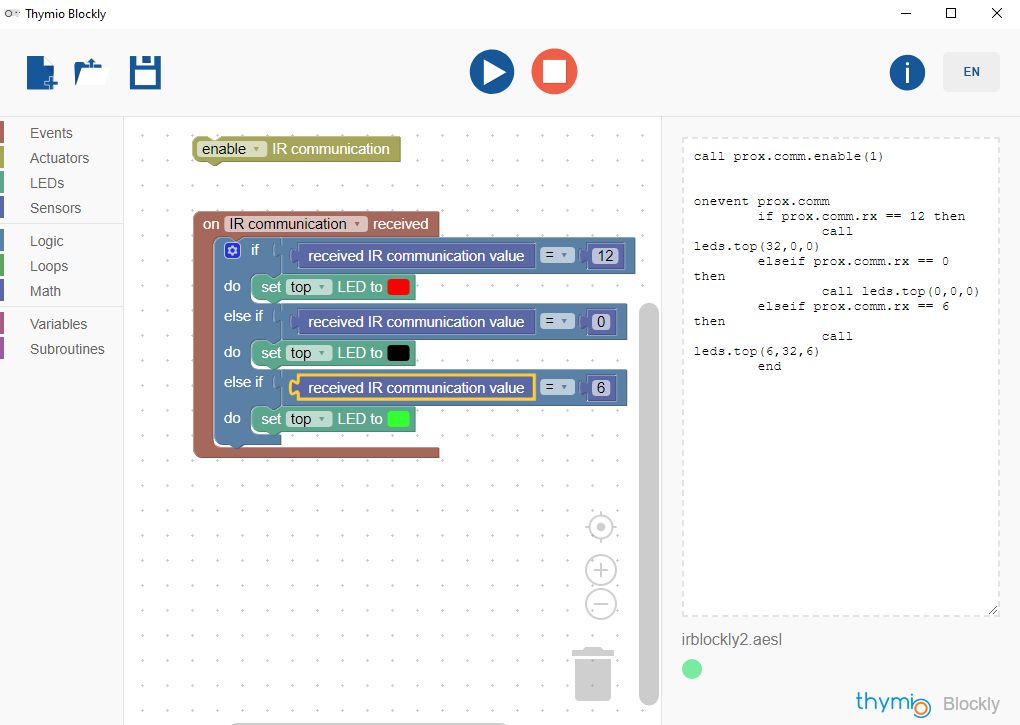
\includegraphics[width=\textwidth]{img/blocklyIR2.png}
		\caption{Un semplice esempio di comunicazione fra due robot}
		\label{blocklyIR2}
	\end{figure}
	
	
\section{Collegare multipli robot}\label{multi-robot}

	È possibile collegare diversi robot allo stesso computer e programmarli in maniera individuale, oppure definire degli eventi comuni.
	
	\begin{figure}[H]
		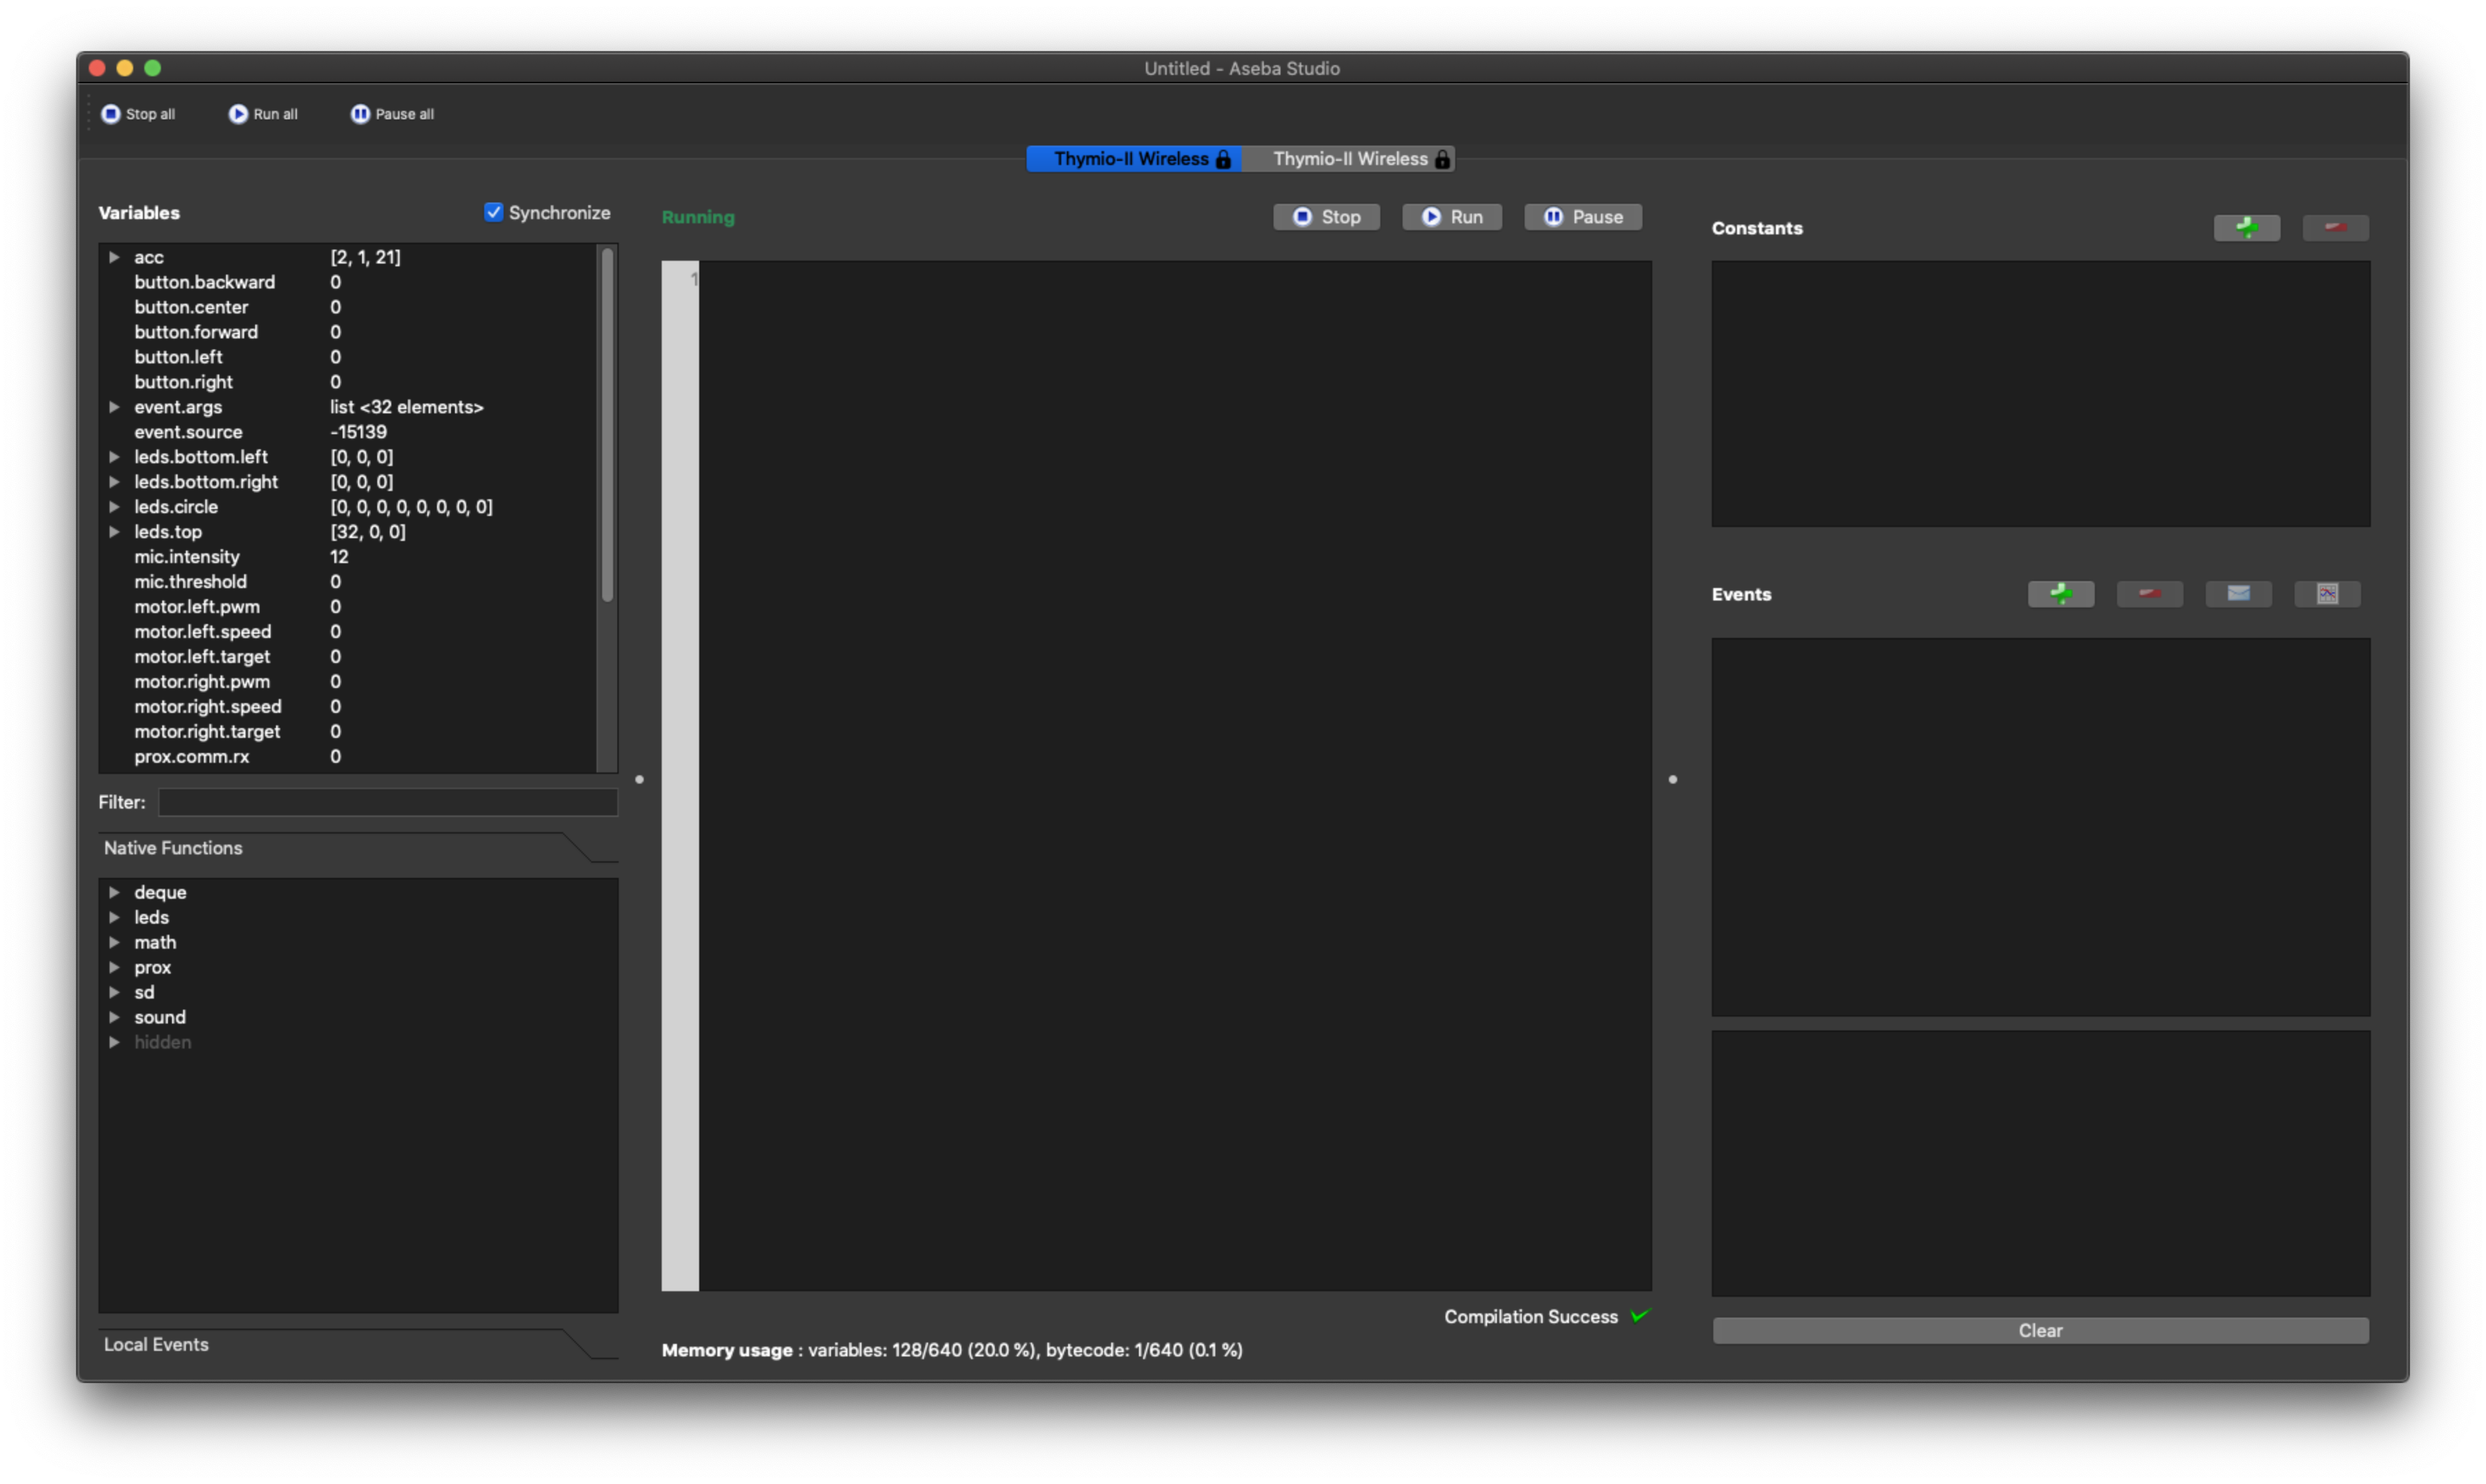
\includegraphics[width=\textwidth]{img/multiRobot.png}
		\caption{Aseba Studio con due robot collegati}
		\label{multiRobot}
	\end{figure}
	
	%TODO istruzioni

		
\section{Aggiornamento del firmware}

	Qualora un robot connesso dovesse avere un firmware non aggiornato, dopo aver selezionato il linguaggio di programmazione desiderato da Thymio Suite un'icona apparirà sul Thymio da aggiornare.
	
	Per installare una versione specifica è necessario scaricare il vecchio pacchetto Aseba 1.6.1 disponibile al link riportato al punto \ref{installation}, sotto la voce \texttt{Scarica una versione precedente}.	
	Recarsi all'indirizzo \url{https://github.com/Mobsya/aseba-target-thymio2/releases} e scaricare il file \texttt{.hex} per la versione più recente. Collegare il robot con il cavo USB e avviare Thymio Firmware Upgrader; scegliere Custom Firmware, selezionare il file appena scaricato e cliccare su Upgrade. 
	
	\textbf{NON} scollegare o spegnere il robot durante la procedura!
	
\end{document}